\documentclass[border=12pt]{standalone}
\usepackage{tikz}
\usetikzlibrary{shapes.geometric, arrows.meta, positioning, calc, fit, backgrounds}
\usepackage{fontspec}
\usepackage{amsmath,amssymb}
\setmainfont{DejaVu Sans}

\begin{document}
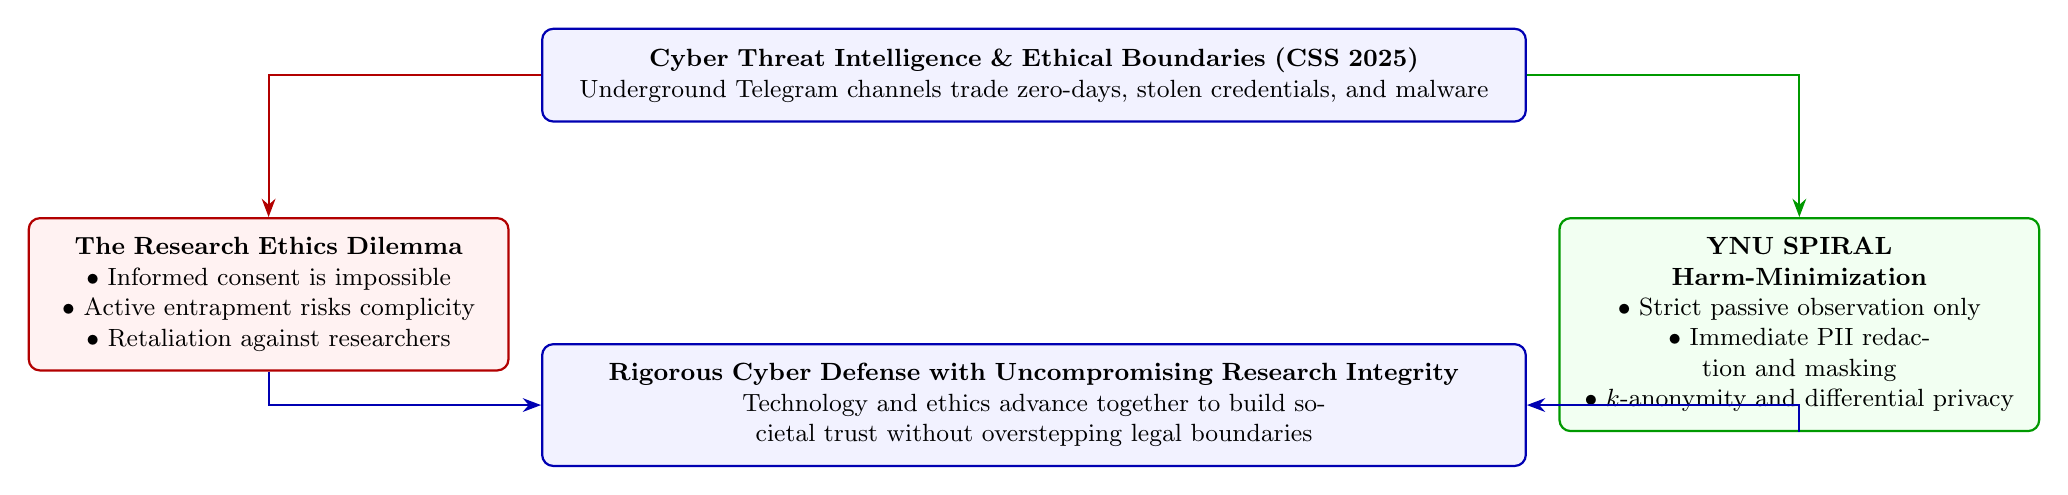
\begin{tikzpicture}[
    font=\small,
    >=Stealth,
    node distance=1.2cm,
    block/.style={rectangle, draw=blue!70!black, fill=blue!5, rounded corners=4pt, thick, align=center, inner sep=7pt},
    alertblock/.style={rectangle, draw=red!70!black, fill=red!5, rounded corners=4pt, thick, align=center, inner sep=7pt},
    greenblock/.style={rectangle, draw=green!60!black, fill=green!5, rounded corners=4pt, thick, align=center, inner sep=7pt},
    amberblock/.style={rectangle, draw=orange!80!black, fill=orange!5, rounded corners=4pt, thick, align=center, inner sep=7pt}
]

\node[block, text width=12cm] (top) {\textbf{Cyber Threat Intelligence \& Ethical Boundaries (CSS 2025)}\\Underground Telegram channels trade zero-days, stolen credentials, and malware};

\node[alertblock, below left=1.2cm and 0.4cm of top, text width=5.6cm] (dilemma) {\textbf{The Research Ethics Dilemma}\\$\bullet$ Informed consent is impossible\\$\bullet$ Active entrapment risks complicity\\$\bullet$ Retaliation against researchers};

\node[greenblock, below right=1.2cm and 0.4cm of top, text width=5.6cm] (framework) {\textbf{YNU SPIRAL Harm-Minimization}\\$\bullet$ Strict passive observation only\\$\bullet$ Immediate PII redaction and masking\\$\bullet$ $k$-anonymity and differential privacy};

\node[block, below=2.8cm of top, text width=12cm] (bottom) {\textbf{Rigorous Cyber Defense with Uncompromising Research Integrity}\\Technology and ethics advance together to build societal trust without overstepping legal boundaries};

\draw[->, thick, red!70!black] (top) -| (dilemma);
\draw[->, thick, green!60!black] (top) -| (framework);
\draw[->, thick, blue!70!black] (dilemma) |- (bottom);
\draw[->, thick, blue!70!black] (framework) |- (bottom);

\end{tikzpicture}
\end{document}
